% Cole Nielsen niels538@umn.edu
% EE 2002 Spring 2015
% Formal Lab Report 1

%----------------------------------------------------------------------------------------
%	PACKAGES AND DOCUMENT CONFIGURATIONS
%----------------------------------------------------------------------------------------

\documentclass[12pt]{article}

\usepackage{circuitikz}
\usepackage{graphicx}
\usepackage{subcaption}
\usepackage[top=1in, bottom= 1in, left=1in, right= 1in]{geometry}
\setlength\parindent{0pt}
\usepackage{fancyhdr}
\pagestyle{fancy}
\usepackage{textcomp}
\usepackage{tikz}
\usepackage{siunitx}
\usepackage{placeins}
\usepackage{titlesec}
\usepackage{cancel} 
\usepackage{tikz}
\usetikzlibrary{shapes.geometric, arrows}
\tikzstyle{box} = [rectangle, rounded corners, minimum width = 3cm, minimum height = 1cm, text centered, draw = black]
\tikzstyle{arrow} = [thick,->,>=stealth]
\usepackage{placeins}

\usepackage{listings}
\usepackage{color}

\definecolor{dkgreen}{rgb}{0,0.6,0}
\definecolor{gray}{rgb}{0.5,0.5,0.5}
\definecolor{mauve}{rgb}{0.58,0,0.82}

\lstset{frame=tb,
  language=C,
  aboveskip=3mm,
  belowskip=3mm,
  showstringspaces=false,
  columns=flexible,
  basicstyle={\small\ttfamily},
  numbers=none,
  numberstyle=\tiny\color{gray},
  keywordstyle=\color{blue},
  commentstyle=\color{dkgreen},
  stringstyle=\color{mauve},
  breaklines=true,
  breakatwhitespace=true,
  tabsize=3
}

%----------------------------------------------------------------------------------------
%	DOCUMENT INFORMATION
%----------------------------------------------------------------------------------------

\title{Lab 1 Report\\ \vspace{0.3 in} EE 4341}

\newcommand{\mymeter}[2]{   	% #1 = name , #2 = rotation angle
 \begin{scope}[transform shape,rotate=#2]
   \draw[thick] (#1)node(){$\mathbf V$} circle (11pt);
   \draw[rotate=45,-latex] (#1)  +(-17pt,0) --+(17pt,0);
 \end{scope}
}
\date{Spring 2016}
\begin{document}
\maketitle 
\begin{center}
 \begin{tabular}{l r}
   Cole \textsc{Nielsen} & niels538@umn.edu\\ 
   Jacob \textsc{Voges}: & voges008@umn.edu\\ 
\end{tabular}
\end{center}
\pagebreak
\pagebreak
%---------------------------------------------------------------------------------------
%----------------------------------------------------------------------------------------
%	Introduction
%----------------------------------------------------------------------------------------
\begin{abstract}
\noindent A LCD display on a PICDEM 2 PLUS board with a PIC18F4520 microcontroller on board was sucessfully programmed to display text sent serially from a PC via RS-232 interface. This was achieved by writing a program to (A) configure the USART (Universal Synchronous/Asynchronous Reciever/Transmitter) of the PIC18F4520 to receive data sent from the PC, and (B) to configure and send the recieved data to the PICDEM 2 PLUS LCD via flipping bits of a port. USART functionality and LCD control was achieved without the use of PIC libraries.
\end{abstract}
\hrulefill
\section{Introduction}
The purpose of this lab was primarily to get the PICDEM 2 LCD display to function, so that it can be used in future labs as a method of receiving data from the microcontroller. Another purpose of this lab was to learn to use the PIC18 USART, which allows for serial communication between the microcontroller and other hardware such as a computer. The use of the USART is useful for debugging and transfering data to and from a microcontroller. In particular the USART is useful when used to communicate to other hardware with the ubiquitous RS-232 interface. This is the communication standard used for this lab. RS-232 works by sending data asynchronously, that is with no clock signal, at a data rate, or \textit{baud rate}, cordinated between two devices. A RS-232 frame (packet) has a standard  sequence, with a start bit, the data message, an optional parity bit and then two stop bits. Both communicating devices know the exact specifics of the sequence so they are able to decode the data. RS-232 was implemented in this lab using the hardware USART peripheral of the PIC18F4520, which will be discussed in the next section. After the USART was implemented, display controller code was written. The LCD is driven by a Hitatchi HD44780U display controller, which takes data asynchronously in a parallel format. The code written implemented a function to bitbang commands and data to the LCD in order to control it and display the USART data. This process will be discussed in greater detail later. 


\section{Implementation}
\subsection*{\normalsize USART}
The USART was configured in two basic parts: an initialization sequence to configure the USART, and a interrupt service routine (ISR) to receive and transmit data. The initialization sequence for transmission was implemented following section 18.2.1 of the PIC18F4520 data sheet, and the receiver from section 18.2.2. Below is the intialization code (part of the initialization() fucntion).
\begin{lstlisting}
	TXSTAbits.SYNC = 0;	// Sync or async operation
	RCSTAbits.SPEN = 1;  // Enable receiver
	TXSTAbits.TXEN = 1;  // Enable transmitter
	RCSTAbits.CREN = 1; //enables rx

	BAUDCONbits.BRG16 = 0; //8 bit BRG reg
	TXSTAbits.BRGH = 1; //baud rate generator speed
	SPBRG = 12;       // Write baudrate to SPBRG

	INTCONbits.GIE = 1; //Global interrupt enable
	INTCONbits.PEIE = 1; //Peripheral interrupt enable

	PIE1bits.RCIE = 1; //interrupt on receive enable (0 - disabled)
	PIE1bits.TXIE = 0;// Interrupt on transmission (0 - disabled)

	TXSTAbits.TX9 = 0; //(0) 8- or (1) 9-bit mode
	RCSTAbits.RX9 = 0;

	TRISCbits.RC6 = 0; //sets Tx to output
	TRISCbits.RC7 = 1; //sets Rx to input
\end{lstlisting}
The first group of statements sets the USART to asynchronous operation and then enables the USART. Next, the baudrate is set to 19200 baud according to the values given in Table 18-3 of the data sheet (4 MHz FOSC). Next interrupts globally and for perifpehals are enabled for the ISR. Finally, the transmit size is set to 8 bit and the port direction for the RX and TX pins are set accoringly. \\\par

The UART ISR is simple, using the interrupt vector associated with all low level interrupts (see code below). When an interrupt is flagged, the ISR executes, and if the flag is because of a USART recieve the data will be stored into the global variable sdata. Reading RCREG clears the flag. The received character in sdata is then writen to the LCD using the WriteByte() function (discussed later) and writen to the USART transmit register TXREG. When written to the transmit register, the data will automatically send, and will show up on the terminal used to send data to the PIC.
\begin{lstlisting}
void low_priority_interrupt(void){
  if (PIR1bits.RCIF){   // if USART receice interrupt
	sdata = RCREG;      // save character received 

	WriteByte(1, sdata);	//write received character to lcd
	TXREG = sdata;			//transmit received characted over UART
  } 
}
\end{lstlisting}
The final and most troublesome part to implement is the code to transmit data from the PIC to the LCD. Since there is no hardware peripheral built into the PIC to do this, it had to be done through software. The LCD has 4 control lines, power, RS (register select) used to select the instruction or data register, R/$\overline{W}$ to read or write to the display registers, and an E which is used to start data read/writes. There are also 8 data line, however only 4 lines where used due to the PCB design. The PCB is layed out where the control lines are the upper nybble of PORTD, and the data lines are the lower nybble. In order to send data or an instruction, the proper combination of RS and R/$\overline{W}$ must be asserted (given in the instruction tables, e.g. Table 12), along with the data to PORTD. E must remain low while changing data. When the data and command lines are asserted, E is strobed High and then low, which initiates the operation on the negative transition of E. Since the data part of the port is only 4 bits, full bytes must be transmitted as two seperate nybbles like previously described. The below diagram illustrates byte sized word transmission in 4-bit mode.
\FloatBarrier
\begin{figure}[h!]
\begin{center}
 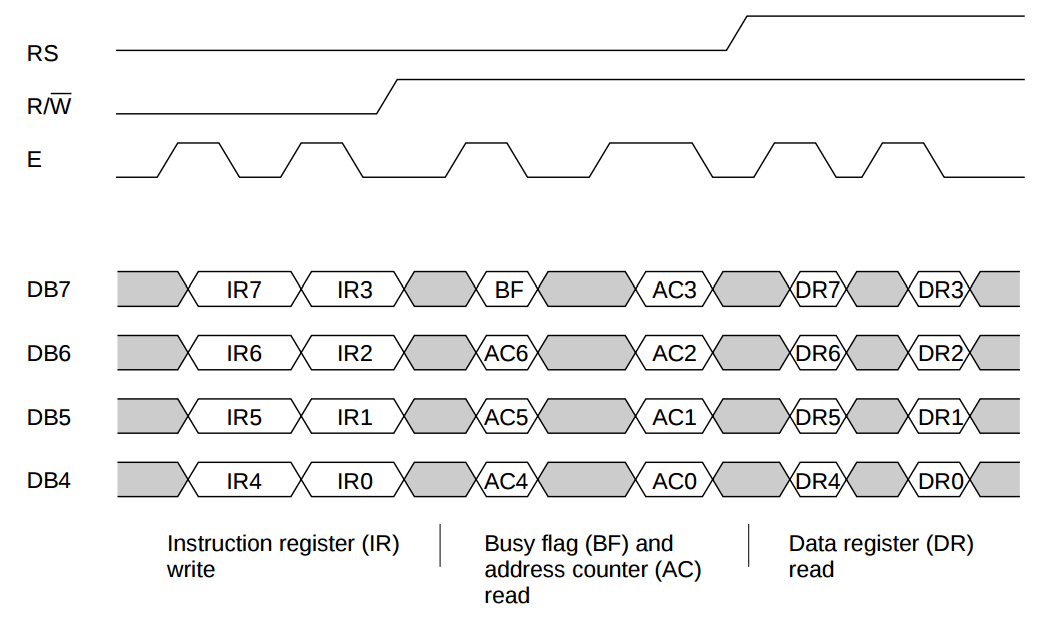
\includegraphics[scale=0.25]{./time.png}
\end{center}
\end{figure}
\FloatBarrier
To transmit data, two functions were written, WriteNybble() and WriteByte() (below in code). WriteNybble() takes two arguments, the first specifying the polarity of RS (if it is data or an instruction), and then a data byte. The lower nybble of the byte is transmitted.
\begin{lstlisting}
void WriteNybble(char RS, char Dat){
	char buf;
	
	if(RS)		//command to be written
		LCD_RS = 1;	//Write data
	else
		LCD_RS = 0; // Instruction reg

	LCD_RW = LCD_EN = 0;// Set write mode

	buf =LATD;                  	// Get high/address nybble
	buf &= 0xF0;                  	// Clear the low nybble
	LATD = buf | (Dat & 0x0F);   	// Combine address nybble and data nybble 
	
	Delay10TCYx(1);		//pulse E line 0-1-0
	LCD_EN = 1;
	Delay10TCYx(1);	
	LCD_EN = 0;
}

void WriteByte(char RS, char Dat){
	WriteNybble(RS, Dat >> 4);            // send high nybble
	Delay100TCYx(2);
	WriteNybble(RS, Dat);                 // send the low nybble
}
\end{lstlisting}
The control lines are first set according to what the RS argument is, and the data and commands lines are written to LATD by combining the upper nybble of LATD with the lower nybble of the data. Finally, E is strobed high for 10 cycles. The WriteByte() function takes the same arguments as WriteNybble(), except both nybbles of the data byte is sent. This is done by calling WriteNybble() within WriteByte() twice, using the upper and lower nybble of the data as the data argument of the two calls.\\\par 
With functions to send data, the LCD is ready to use. Using the LCD requires an initialization sequence shown below (part of the initialize() function):
\begin{lstlisting}
	PORTDbits.RD7 = 1; 	//turn on LCD
	Delay10KTCYx(6);	//wait >15ms for LCD to stabilize

	WriteNybble(0,0x03); //send 8 bit function set
	Delay10KTCYx(2);  	//wait >4.1ms
	WriteNybble(0,0x03); //repeat 8 bit command
	Delay100TCYx(4);	//wait > 100us
	WriteNybble(0,0x03); //repeat 8 bit command again
	Delay100TCYx(2);	//wait ~50us

	//set up sequence
	WriteNybble(0,0x02); //set to 4 bit mode
	Delay100TCYx(2);	//wait ~50us
	WriteByte(0,0x28); //function set
	Delay100TCYx(2);	//wait ~50us
	WriteByte(0,0x0E); //turn display on
	Delay100TCYx(2);	//wait ~50us
	WriteByte(0,0x06); //entry mode set to shift cursor right
	Delay100TCYx(2);	//wait ~50us
}
\end{lstlisting}
This first two parts of the initializtion sequence is based on the chart given in figure 26 of the Hitatchi datasheet. The second part is based from Table 12 of the same datasheet. The comments are self explainatory. The last remaining part of the code is the main function which only has a call to the initialization function, and then a empty while loop to keep the MCU busy.
\section{Summary}
The outcome of this lab was a functioning code for USART communication using the PIC18, as well as code to drive the PICDEM LCD, both of which can be used in future labs. Better understanding of the PIC18, LCDs and UARTs was also gained, mostly through mistakes made. One of the first mistakes made was to not set the config bits to select the clock source. This was discovered as the MCU would do nothing at power up, so the config bits were set for the XT clock to resolve this. A second issue was that the USART ISR would keep sending a received character back to the computer. This was because the TXREG was written outside of the receive if statement of the ISR, and the TXIF flag was set, so the flag would go off and the ISR would keep executing and resending the character and so on. This was fixed by moving the TXREG write into the receive interrupt if statement and disabling TX interrupt. A final issue encountered is the LCD would not display anything. The issue was discovered to be that the startup sequence of figure 26 of the Hitatchi datasheet was not implemented after reading the datasheet closely. This was fixed by implementing the startup sequence. Below: working code demo.
\FloatBarrier
\begin{figure}[h!]
\begin{center}
 \includegraphics[scale=0.07]{./demo.jpg}
\end{center}
\end{figure}
\FloatBarrier

\end{document}
